\chapter{Remote Method Invocation}
\section{Overview}
In modern, large distributed systems, nodes can be running in processes on several different physical machines. Using the Java Remote Method Invocation this can be done opaquely from the user. 

The Java RMI makes this possible. 

\section{Java RMI}

\subsection{Java Virtual Machine}
The Java Virtual Machine is a component that can execute Java bytecode. It is has an implementation on almost every platform and makes it possible to reuse your code on all these platforms. It JIT compiles the code to enable garbage collection and runtime code verification, so that programmer errors and safety isssues is avoided.
Java bytecode and the JVM is analogous to Microsoft's .NET managed code and CLR (Common Language Runtime).

\subsection{Remote Method Invocation}

Remote Method invocation is an API integrated in the Java Virtual Machine which allows for remote procedure calls in an object-orientated manner. This is done by serializing java classes and transfering these to the remote location.

RMI is not to be confused with RPC (Remote procedure calls) since these are not object orientated.

Java RMI consists of three layers::

The \textbf{Stub and skeleton layer} are placed on either side of the whole network and transfer area. On the client side, a stub is created when a object is requested from the registry. When the client invokes a method on the stub, it communicates with a skeleton on the server side, which invokes the remote object.

The \textbf{Remote Reference layer} can be considered a middleware between the stub/skeleton layer and the transport layer. It handles references of remote objects, and manages creation, duplication and destruction of remote these objects. A Remote Reference manager (which is a sort of "controller" in this layer) is present both at the client and server side.

The \textbf{Transport layer} is responsible for network transfer. Here the TCP/IP connection is implemented. Here, the endpoints and incoming and outgoing connections is managed.

The coupling between the three layers is shown below:

\begin{center}
	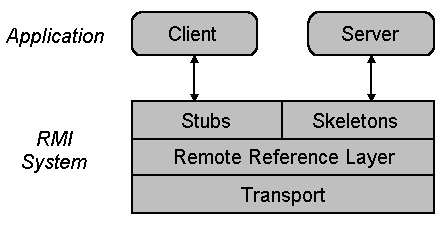
\includegraphics[scale=1.0]{RMI_layers.png}
    \captionof{figure}{RMI layers \cite{carleton}.}
\end{center}

\subsection{Serialization}
To be able to send data to another component / computer, Java RMI needs to serialize the data when it is send and then deserialize it when it is received. 
Serialization means to convert some data into sequence of bytes that holds the original values and information on the source eg what kind of object it is. It should also be possible to convert it back into the original data at any time (deserialize). This concept is often used when data is saved into a file or database or when data is transferred over a network.

\subsection{The RMI Registry}

\section{Leader election}
\subsection{Overview}

\subsection{Leader Election}

\subsection{Bully Election}
The bully election algorithm basically elects the process with biggest process id as the new leader when the old leader is terminated. 
If a process takes contact to the leader and doesn't get a response, it will then start a leader election by asking all processes with an id greater than its own, if they will be the leader. These processes will then reply if they are active that they will take over by continuing the algorithm. 

If a process doesn't get an answer, then it is elected as the new leader and will state this to all other processes.

This algorithm is very ineffective because you will quickly get a very high number of requests when all processes must ask all other processes with a higher id.

\subsection{Ring Election}
Ring election is , as the name says, leader election based on a ring. Contrary to Bully election, each note only communicates with the next in line.

Consider this figure:

\begin{center}
	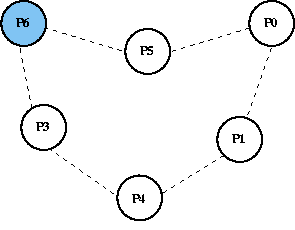
\includegraphics[scale=1.0]{RingElection_1.png}
    \captionof{figure}{Ring Leader Election \cite{colostate_RingElec}.}
\end{center}

Node number 6 crashes out, which leaves the system without a leader. When node number 3 tries to contact node 6, it realises that the leader has gone down, and it initialises a new election. A message is passed around the ring, and each node appends its own id to the list. When the message returns to node 3, it determines that it's id is already in the message, and the ring must be complete. Node 3 now determines the new leader. A message is sent around the ring, notifying everyone (including the new leader) who is the new leader. When this message reaches node 3 again, the node knows it has to stop it.\footcite{colostate_RingElec}

\begin{center}
	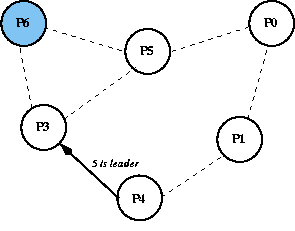
\includegraphics[scale=1.0]{RingElection_2.png}
    \captionof{figure}{Passing new leader message around \cite{DesignPatterns}}
\end{center} 
